\chaptertitle{3}{要多少钱，才能实现财务自由}
\setcounter{figure}{0}\setcounter{table}{0}
我们在上一章讲过，人力资产也可以产生现金流，那我们就先来算一算，自己值多少钱。

\subsection{我们自己值多少钱}
{\heiti 人力资产，是每个人最大的一笔资本}

我们自己，也是一项可以产生现金流的资产。

古人经常说，养儿防老。在传统社会，没有医疗、养老等保障体系。分散老龄化风险的一个方法，就是多生几个孩子，每个孩子都可以通过劳动获得食品等生活物资，这样自己到年纪大了劳动能力下降的时候，孩子就可以分担自己的养老压力。

孩子在某种意义上，就是一项资产，可以为老年人提供现金流。

到了现代社会，医疗、养老体系已经健全。社会分工明确，绝大部分人都有自己的工作，可以通过劳动来获取工资等现金流收入。这种情况下，我们每个人都是一项可以产生现金流的资产。

比如说一个刚毕业的大学生，他手里可能没有多少钱，但是并不能说他什么资产都没有，因为他本身就是一项资产。他可以去工作赚取工资收入。

对年轻人来说，人力资产是很重要的，可以说是最大的一笔资本。如何去计算人力资产的价值呢？

这里有一个参考。北京市交通事故赔偿标准提到“死亡赔偿金”：城镇居民死亡赔偿金，按照上一年的人均可支配收入的20倍计算。

比如说2016年北京地区，城镇居民人均可支配收入是57275元。那2017年，死亡赔偿金就是57275×20=1145500元。如果一个北京地区的普通成年人不幸在交通事故中死亡，其本身价值就是按这个数字赔偿。

这里的20这个数字挺有意思，它实际上就是投资领域经常提到的市盈率。假设一个人年收入是5万元，那这个人的“市值”就是5万×20=100万元。国家认为一个人的市盈率平均应该按照20倍计算，这个值挺有参考意义。关于市盈率，在本书后面还会有详细介绍。

大家也可以用这种方法，计算一下自己一份工作的价值。刚开始上班的时候可能工资还不稳定，可以以单位老同事的平均收入为基准。比如说，税后年收入稳定在20万元，如果要一直从事这份工作，那这份工作的价值差不多就是：20万×20=400万元。

{\heiti 稳定工作=优质的“债券类资产”}

一份稳定的工作，本身就是一项优质的“债券类资产”。

比如说有两个人，一个有100万元存款，但是没有工作或者其他现金流收入；另外一个有50万元存款，但是有一份年收入10万元的工作。

前者因为没有现金流收入，其人力资本没有体现，是闲置的，而后者实际上是“50万元的股票资产+200万元的人力资产”。在不考虑其他因素的情况下，后者的安全感应该会比前者更强。

这也是家长总是期盼孩子能有一份好工作的原因。好工作可以增强人力资产的价值和现金流。

{\heiti 如何提升人力资产的价值}

那有哪些因素，影响了我们这个人力资产的价值呢？

比较神奇的是，我们自身这项人力资产，是可以凭借主观能动性来提升价值的。

在股票市场或者其他投资领域，我们再怎么努力，也很难凭主观意愿改变某只股票的走势，通常都是投资之后耐心等待。但是我们自身这项人力资产的价值，可以凭借我们的努力去提升。

（1）我们之所以寒窗苦读十几年甚至二十几年，原因在于教育是最好的一笔投资，它可以非常明显地提升我们自身这项人力资产的价值。

1992年诺贝尔经济学奖获得者加里·贝克尔（Gary Becker）教授，是首位把人力看作资产的学者。他很重要的一个理论就是“教育的投资回报率是巨大的，投入时间和金钱提高人的受教育程度是非常值得的”。

通过对美国市场的研究，投资到一个本科学历上的钱，年化收益率达到了15\%！这是考虑了通货膨胀因素之后的真实收益率，比股票、房产等的长期收益率还要高。中国也是如此。

这也是我们要好好学习的原因。学历越高，平均收入越高；学校越好，平均收入越高。不排除个别名校毕业生发展不好，收入不高，但是从整体上来说，这个逻辑是成立的。

美国大学学费那么高，但很多人不惜贷款也要上大学。他们不是傻瓜，是因为他们知道这笔投资的回报率高得惊人，远比大多数资产的回报率要高，自然抢着去投资。

（2）上班后，努力学习、认真工作也可以显著提升收入。

很多单位，如果员工愿意去考取相关证书，培训费、报名费单位都会报销。有了这些证书后评职称会更容易，同样的工龄，收入也会显著提升，带动个人价值的提升。

当然，我们可能发现自己不喜欢正在从事的工作，或者找到更适合自己的工作，这时可以换工作。换工作在现代社会是一件很正常的事情。

一个好的学历、一份好的工作，会大大提升人力资产的长期价值。所以，家长才愿意在孩子的初高中教育上投入重金，考研辅导班、公考国考辅导班才会非常火爆。这真的是有投资价值的。

{\heiti 人力资产的风险}

但是人力资产也是有风险的。它主要来自两方面：一种是意外风险，人力资产本身会面对各种复杂的情况，特别是遇到一些疾病、意外等风险；另一种是时间风险，我们的劳动能力会随着时间的推移逐渐下降。

不过好在，这两种风险在现代社会都有办法规避。

第一种风险，主要是意外、疾病等导致的。比如说不幸遇到车祸、身染重疾。这种情况下我们无法到岗工作，会对我们的劳动能力产生非常大的影响。

对于这些风险，我们可以依靠保险来化解。例如不幸得了癌症重疾，不仅无法上班获得收入，还需要家庭花费大量的钱去治疗，严重拖累家庭的生活质量。但是如果配置了重疾险，确诊重疾险里所包含的重疾，就可以先行得到一大笔赔付，抵抗这种风险。意外、重疾、医疗开销等风险，都可以通过保险来对冲。不过这些风险也不是每个人都会遇到的。

第二种风险，则是所有人都会遇到的，那就是随时间的推移，我们都会衰老，劳动能力会下降。

二十多岁的时候，我们熬通宵易如反掌，第二天照样生龙活虎地学习工作。但四十多岁的时候，熬一夜就得好几天才能缓过来。到了五六十岁，高强度的工作就无法胜任了。

年纪越大，我们劳动能力越低。与之对应的，是我们的人力资产的现金流，也就是工资，也有可能下滑。

特别是退休之后，退休金相比还在上班时的工资收入，是要打一个折扣的。

不过有退休金和养老金，这还算不错的了。如果是个体户或农民，年纪大了之后可能不仅收入下滑，而且没有足够的退休金和养老金来负担老年生活。

如果人力资产是家庭资产的主力，那我们的家庭就必然会面对这样的风险。

{\heiti 如何化解人力资产的时间风险}

这是社会和国家的一个大问题。

大多数年轻人需要依靠自己的体力或者努力工作来赚取工资收入，这其实就是把自己这项人力资产运作起来产生现金流。

我们可以利用得到的现金流逐渐配置各种能产生现金流的资产。例如有的人会把工资存入银行，买银行理财产品；有的人会用工资买股票或基金；有的人会多买几套房子，预备养老。不同人的选择不同。

等到积累的资产足够多，这些资产产生的现金流可以覆盖家庭日常生活的开销，我们也就实现财务自由了。

这就是用定投来化解人力资产的时间风险。

这个过程会持续几十年的时间。早期我们的家庭资产中人力资产是主要部分，但随着定投的延续，人力资产产生的现金流就逐步变成其他资产。最终当我们积累了足够多的其他资产，而这些资产产生的现金流足够我们的生活所需时，我们也就可以退休了。如果做好投资的话，这个过程需要的时间会大大缩短。

我们也就明白了为何定投是分批投入的，因为资产产生现金流需要时间。人力资产产生的现金流，也就是工资现金流，通常是定期发放的，所以大部分定投也是定期的。

定投的实质，就是把人力资产定期转化为其他资产。所以只要我们还在工作，还在用人力资产产生现金流，就要面对如何定投的问题。

所以从某种意义上来说，每一个劳动者都需要考虑定投的问题，只不过定投的品种、定投的操作各有不同。

\subsection{延迟退休，你准备好了吗}
这两年关于延迟退休有不少新闻，有的官员建议延长退休年龄。

当然，这个提议有很多人反对。但是从另一个角度想一想，退休年龄的延长，其实是必然的。

{\heiti 延迟退休，是未来的趋势}

如果去日本旅游，我们会看到很多年纪非常大的人还在工作，很多海外的航班上也没有年轻的空姐，更多的是一些年纪较大的空姐。

这跟咱们国内的现状很不一样。国内目前很多退休的人都领着退休金去各地旅游，或是享受天伦之乐。像之前螺丝钉去三亚的时候，就看到在海边休闲散步的大部分都是老年人。

但其实，我们人类的寿命是在不断延长的。过去，60岁已经是高寿了，但现在60岁退休之后，一般人还可以继续生活几十年。

几十年后，70岁的人身体素质就像现在60岁的人一样，人类的平均寿命可能会延长到百岁以上。

如果依靠现有的年轻人的工作，其实是负担不起这么多老年人退休后的需求的。所以延迟退休是未来的趋势，甚至会变成日本那样，很多七八十岁的人还在工作。

我们该如何去应对呢？这其实需要我们先回答这个问题：养老靠什么？

{\heiti 农耕时代，养老主要靠儿女}

在不同的时期，养老的依靠是不同的。

在农耕时代，养老主要靠子女、靠亲朋。

如果一个人从事的是体力劳动，或者是对身体硬件条件有要求的工作，可能工作到60岁就需要退休了。毕竟年龄不饶人，身体素质下降是每个人都需要面对的。

有句老话叫：养儿防老。

在农耕时代，多一个儿子，就是多一份劳动力。这个劳动力，可以通过劳动来种植作物、收获粮食，也算是一种可以产生现金流的资产。

因此，只要多生几个孩子，自己的晚年生活就基本上有保障了。所以农耕时代的人，就是努力劳动、多生孩子，在老年靠孩子来养活自己。

也有的地方养老采用的是宗族制度，即依靠家族亲戚之间互相帮助。直到今天，还有很多地方延续这种方式。

{\heiti 现代社会，养老靠的是资产}

不过在现代社会，纯粹的体力劳动明显减少，很多人从事的是脑力劳动，那其实60岁以上的人还是可以继续工作的。

所以，现代社会养老依靠的是能产生现金流的资产。

比如说“股神”巴菲特，在八九十岁的高龄，仍然每天积极学习投资知识、阅读各种信息，每年股东大会还可以一讲讲一天。

巴菲特的工作并不太依靠体力，更多的是根据投资知识和经验来调配资产，买入低估的、能产生现金流的资产。其绝大多数财富都是60岁之后赚到的。

这是因为投资有很强的复利效应，哪怕是多工作10年，也可以让财富有非常明显的增长。并且后一个10年里积累的财富，可能是上一个10年的很多倍。

不是没有比巴菲特投资收益高的投资者，但是，比巴菲特收益更高，还比巴菲特活得时间更长、工作时间更久的投资者，真是非常稀少。

对巴菲特来说，投资是他的爱好，只要身体条件允许，他会一直工作下去。而且工作对巴菲特来说是一种乐趣，巴菲特说他自己是“跳着踢踏舞来上班”。

不过对大多数人来说，年轻的时候都需要努力工作，依靠自己的体力劳动或者脑力劳动来赚取收入。

这其实是把自己这项人力资产运作起来并产生源源不断的现金流。得到的现金流，我们可以用来配置各种优质的资产，例如社会上优质的股票资产、优质的房地产资产等。

这些资产，可以进一步产生现金流，但这是被动的现金流，不再需要我们辛苦工作就可以获得。等这些能产生被动现金流的资产积累得足够多，且这些被动现金流可以覆盖家庭的支出时，那我们之后的生活就不用太担心了。

{\heiti 持有优质资产，是应对延迟退休最好的办法}

其实，这也就是财务自由的意义所在。不需要辛苦工作产生现金流，而是通过资产来获得被动现金流，满足自己和家庭的生活所需。同时，还可以选择去做一些自己想做的事情。

即使过了60岁，只要身体条件允许，我们可以继续做自己喜欢的事情，也有足够的财力来自由选择是不是要一直做下去。

持有优质资产，是应对老龄化和延迟退休的最好方法。

这种情况下，我们变成了时间的朋友，活得越久越有优势。因为资产会以复利的形式增值，时间越长，复利的威力越大。

长期投资，最后往往拼的是谁活得更长。掌握优质资产的投资方法，能让自己有更大的选择空间。

\subsection{攒多少资产，才能实现财务自由}
那具体需要多少资产，才能实现财务自由呢？

{\heiti 财务自由的4\%法则}

如果依靠退休金和养老金来养老，我们只需认真工作到退休年龄即可。至于退休金和养老金是怎么投资的、现金流如何发放、如何抵御通货膨胀的侵蚀，这些都不需要我们操心，我们只需要做好本职工作即可。

但如果我们想要实现更高质量的财务自由，就得解决一个问题：我们需要攒多少资产才够呢？

这是可以量化出来的。有一个比较通用的方法：4\%法则。

4\%法则是麻省理工学院的学者威廉·班根（William Bengen）在1994年提出的理论。通过投资一组资产，每年从退休金中提取不超过4\%的金额用来支付生活所需，那直到自己去世，退休金都花不完。因为，资产自己会增值。

换句话说，如果一年需要40万元的开销，那就需要40万元/4\%=1000万元。把这1000万元投资到一组资产上，每年提取不超过4\%的金额，就可以满足一年40万元的生活开销，实现财务自由。

所以我们可以先计算一下，我们想要实现什么段位的财务自由，要实现这个段位的财务自由，家庭一年需要多少开销，再反过来推算需要多少资产。

但是这项资产，并不是什么资产都可以，这项资产的长期收益率必须超过4\%，否则不足以支撑每年提取4\%的金额。另外，这项资产得以能够抵御通货膨胀的资产为主。

{\heiti 要赚多少，财富才不会缩水}

为什么现代很多中产家庭会缺少安全感呢？原因在于现有的财富可能会受到通货膨胀的侵蚀而缩水。

其实钱的数量本身，不太容易给人带来安全感。因为货币在贬值，并不是说现在一个月赚2万元就安全了。

比如说20世纪90年代的时候，大部分人的月工资不到1000元，如果有一份工作的月工资有3000元，那人们的安全感是十足的。但现在，月收入3000元满足不了大部分人的需求。

同样地，若干年后，人均月工资可能到了20万元甚至更高，2万元又不能满足人们的需求了。一个静态的收入数字是无法给人带来安全感的，因为现金是没有办法抵抗通货膨胀的。

什么是通货膨胀呢？

一些书里会告诉你，通货膨胀率看的是CPI，也就是居民消费价格指数。这也是一个指数，只不过跟股票指数不同。这是统计我们普通家庭平时购买的居民食品饮料、能源等消费品或者服务项目的市场零售价格的指数。

最近几年，按照国内的统计，CPI同比增长一年为2\%～3\%。也就是说，我们日常生活的居民物价，上涨速度是每年2\%～3\%。

按理说，我们投资的收益率，跑赢CPI的增长速度，就算是跑赢通货膨胀了。

如果按照上面这个标准，跑赢通货膨胀并不难实现，买点理财产品就可以做到。

不过这个数字，肯定跟大家的实际体验有很大差别。

为什么呢？

这是因为CPI可以被看作“必需消费通货膨胀率”。跑赢了CPI，我们就能够活下去。但是如果想要更好的生活质量，其实需要跑赢的是“可选消费通货膨胀率”。

比如说任何一个社会，优质的教育、医疗等资源的价格增长速度一定是大幅高于CPI的。因为整个社会都需要这些资源，大家互相竞争，就会推高这些资源的价格。这些消费的价格增长速度，比3\%要高不少。

家里有孩子的朋友一定深有感触，因为给孩子的补课费用一年比一年高。虽然学校的学费可能增长并不快，但实际上，培养出一个985或者211重点学校的本科生，所需要的开销的增长速度是远高于CPI的。这些稀缺资源价格的增长速度，通常跟M2增速有关系。

M2是广义货币的量，比如说我们的存款、证券保证金、公积金等，都算是广义货币。M2的增长速度，代表一个社会广义货币的增长速度。

俗话说，水涨船高，货币供应量增加了，市场上的钱多了，物价也会上涨。涨价很大一部分就是因为货币流入并推高社会稀缺资源的价格上涨。

M2的增长速度，在十几年前长期保持在两位数。最近几年有所下降，最近三年M2的同比增长速度保持在8\%～9\%。

社会上稀缺资源价格的增长速度，通常跟M2的增长速度有很大关系。

注意，这里是有很大的关系，但并不是说这些稀缺资源价格的增长速度正好等于M2的增长速度。这些稀缺资源，包括优质的学区房、北京或上海等一线城市户口、培养一个重点大学本科生的教育资源等。

例如之前网上流传一个上海地区的“牛娃”培养日记。想要孩子上好大学，就得上好高中；想要上好高中，就得上好小学；想要上好小学，就得上好幼儿园。最后要从孩子出生就开始抓起，甚至有的家长从备孕就开始准备了。

高等教育的成本，远不止学校收取的学费。因为优质教育资源是稀缺的，想要得到它，需要跟社会上其他人竞争。

跟谁竞争呢？

跟社会上更有钱的家庭竞争。这些家庭受益于货币增发，家庭资产增值速度比较快。这样最终会导致稀缺资源价格的增长速度是跟M2增长速度匹配的，甚至可能要高于M2增长速度，而不是跟上面说的与CPI增长速度匹配。

我们家庭实际面临的通货膨胀率介于这两者之间，为3\%～9\%。因为我们的消费是由必需消费和可选消费组成的。日常衣食住行有，教育、医疗等也有，并不纯粹由某一方面来构成。

并且，不同家庭所处的时间段不同，花销的侧重点也不同。比如说年轻的时候，需要养孩子，那我们需要的投资回报率就要更高一些；当退休之后，孩子也长大自立了，自己又没有特殊需求的话，那所需的投资回报率可以低点儿。

通常来说，我们投资长期债券基金，包括理财产品，是可以跑赢CPI的。债券基金的长期平均收益率在6\%上下。也就是说，掌握了债券基金的投资技巧，可以保证我们的基本生活质量。但如果想要过上高质量的生活，那么单靠债券基金就不行了，最好是要有收益率能匹配甚至高于M2增长速度的资产。

{\heiti 哪些资产可以抵抗通货膨胀}

什么样的资产可以带来安全感呢？

其实持有优质的可以抵抗通货膨胀的资产，是最容易带来安全感的。例如在一二线城市有很多套没有贷款的房子，有一家盈利不错的公司，或者有一份在大型互联网公司的工作且持有很多股权。我们认真工作，赚取工资现金流然后把这些工资现金流，尽可能多地换成优质的可以抵抗通货膨胀的资产。长此以往，我们手里的优质资产会越来越多，这些资产会帮我们赚钱。最后，我们手里会持有很大比例的资产，即使不靠人力资产赚工资，也可以很好地生活下去，完成从无产者到有产者的过程。

这是让我们的生活过得越来越轻松的好方法：持有优质的可以抵抗通货膨胀的资产。

而可以抗通货膨胀的资产主要有三类：人力资产、房地产、股票资产。

人力资产是可以抗通货膨胀的。比如说2000年的时候，城镇居民人均可支配年收入是6280元，平均到一个月是523元。到2017年，城镇居民人均可支配年收入是36396元，平均到一个月是3033元。人力资产的价值以10\%左右的年均增速上涨。所以未来高校毕业生的薪酬和期望的薪酬，也是会不断上涨的。当然以上数字只是一个平均值，具体到不同专业和能力的毕业生，差别还是很大的，还是要自己去努力。

人力资产以工资的形式体现。所以最后，要实现高质量的财务自由，需要积累的资产主要就是房地产和股票资产了。

房地产是非标准化的资产，各地区的房地产投资价值、政策各有不同，即使同一城市，不同区域的发展也有很大区别。甚至同一条街上不同小区的房价，10年里的涨幅可能也会差2～3倍。一二线城市和三四线城市房地产投资策略也有很大的差别。比如北京很多二手楼盘还是挺受欢迎的，但是在三四线城市，这种楼盘基本无人问津，因为有大量新楼盘可供挑选。再比如北方有的地区一楼很受欢迎，因为可以带个小院子，但在南方，一楼因为太潮湿反而不好，不能一概而论。

这种非标准化的资产，不在本书的探讨范围内。本书主要以标准化的股票资产，包括股票基金等作为定投的研究对象。这是每位普通投资者都可以平等地接触到的可抵抗通货膨胀的资产。

其实跑赢通货膨胀的方式还有很多种，比如成功创业、提升工资收入的增速。

不过以上方式通常比较难实现，这也不要紧，我们还可以投资低估的指数基金。长期来看，低估指数基金的收益是可以跑赢通货膨胀的。这也是我们做好指数基金定投的一个原因。这本书的目的，也就是帮助大家通过定投来更好地实现高质量的财务自由。

\subsection{财务自由，不等于什么都不做}
{\kaishu 钉大，我有一笔资金在打理。按照您的方法，我相信10\%的收益率的话，该收益会超过我现在工作的收入。目前我对工作的兴趣不大，但对财务自由是真爱，所以打算彻底专注于理财。但是，一旦没有工作，这些理财收益可能就需要被用于生活各种支出了。我感觉有些矛盾，想听听您的意见。}

很多人理解的财务自由，是当被动收入满足生活开支后，就什么事都不干了，开开心心地天天玩儿。但是实际上并不是这样。人是一种社交动物，如果没事干，会很空虚的。这跟是不是财务自由没关系，人需要给自己找事情做。

{\heiti 财务自由，也要给自己找事情做}

螺丝钉离职的时候没有在财务自由的状态，不过提前过了一段离职后的自由时光。刚开始是很爽的，感觉像是放了一个长假，但是过了一两个月之后，就很难受了。

没有工作的朋友，极易与社会脱节，而且没有自制力的话，很容易堕落，生活没有规律。

所以即便是财务自由，也要给自己找事情做。

{\heiti 人类需求的5个层次}

马斯洛（Maslow）把人类的需求分成5个层次：生理需求、安全需求、爱和归属感、尊重和自我实现，由较低层次到较高层次依次排列。

\begin{figure}[htbp]
\centering
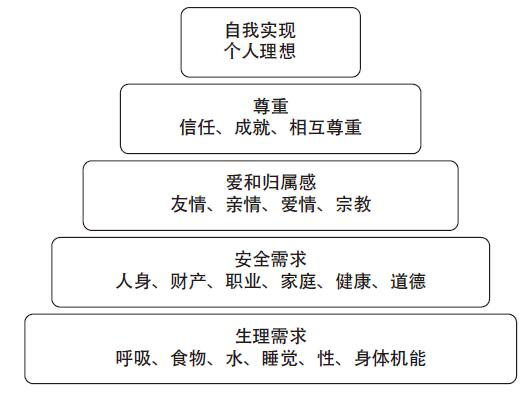
\includegraphics[width=\textwidth,height=0.82\textheight,keepaspectratio]{figure/图3.1.png}
\caption{马斯洛需求层次理论}\label{fig:3-1}
\end{figure}

吃喝等是基本的生理需求，这是人要活下去所必需的。

安全需求，包括对人身安全、家庭安全、工作稳定、财产安全等的需求。我们追求稳定的工作和家庭生活，就是为了满足安全需求。例如许多中产家庭经常很焦虑，原因在于他们对家庭财产没有安全感，担心其被通货膨胀等因素侵蚀。如果没有实现财务自由，那他们的安全需求是无法被满足的。\\

爱和归属感，这跟财务状况关系不大，主要来自家人、亲朋、爱人。再有钱的人，也渴望爱情、亲情和友情。很多有钱人的家庭生活一塌糊涂，爱和归属感都没有被满足。

尊重，人需要被社会认可。一些暴发户会在公开场合炫耀自己的财富，其实就是希望自己能够被社会认可。实现财务自由之后，如果不与社会接触，也很难得到别人的尊重和认可。很多志愿者不计报酬地帮助别人，其实也是为了得到别人的尊重和认可。

最后是自我实现。内心有梦想，跟有多少钱没关系。很多成功的企业家已经有巨额的财富、美满的家庭、社会的尊重了，但是他们内心想要做的事情还没做好，他们还会坚持做下去。

对螺丝钉来说，即便未来实现财务自由，也不会停下来什么都不做。让更多人认识到指数基金投资的好处，普及指数基金投资，甚至最后成立属于自己的基金公司，这些都是尊重和自我实现的需求。

{\heiti 实现了财务自由，只是完成了人生目标的一小半}

实现了财务自由，我们仍然需要去经营好家庭和亲朋的关系，满足爱与归属感的需求，需要去帮助别人，或者被别人需要和认可，满足尊重的需求，需要有一个梦想，满足内心自我实现的需求。

实现了财务自由，只是完成了人生目标的一小半。钱是一个好工具，但不应该是我们内心真实的需求，我们还需要继续挖掘我们的内心，找到真实的自我，看看自己真正想要的是什么。不过，财务自由可以让我们更好地找到真实的自我。

{\heiti 投资者笔记}

\begin{itemize}
\item {\kaishu 对年轻人来说，人力资产是很重要的，可以说是最大的一笔资产。而一个好的学历、一份好的工作，会大大提升人力资产的长期价值。}
\item {\kaishu 定投的实质，就是把人力资产定期转化为其他资产。}
\item {\kaishu 农耕时代，养老主要靠儿女；现代社会，养老靠的是资产。持有优质资产，是应对老龄化和延迟退休的最好方法。}
\item {\kaishu 优质的可以抵抗通货膨胀的资产，主要是这三类：人力资产、房地产、股票资产。}
\end{itemize}

